% LaTeX .tex
% Example for the proceedings of the  25th International Congress of Mechanical Engineering
% COBEM 2019
% October, 20-25, 2019, Uberlândia, MG, Brazil
% Based on the template of the proceedings of COBEM2015 and COBEM2017

\documentclass[10pt,fleqn,a4paper,twoside]{article}
\usepackage{abcm}
\def\shortauthor{F. Author, S. Author and T. Author (update this heading accordingly)}
\def\shorttitle{Paper Short Title (First Letters Uppercase, make sure it fits in one line)}
\usepackage{subcaption}
\captionsetup{compatibility=false}
\usepackage{blindtext}
\begin{document}
\fphead
\hspace*{-2.5mm}\begin{tabular}{||p{\textwidth}}
\begin{center}
\vspace{-4mm}
\title{Study of mechanical properties of parts fabricated with PETG via fused deposition modeling}
\end{center}
\authors{Ma\'ira Fernanda Oliveira de Miranda} \\
\authors{Felipe Jose Oliveira Ribeiro} \\
\authors{Alexandre Zuquete Guarato}\\
\institution{Federal University of Uberl\^andia (UFU), Av. Jo\~ao Naves de \'Avila, 2121, Campos Santa M\^onica, Uberl\^andia, MG } \\
\institution{mairaf\_miranda@hotmail.com} \\
\institution{feliperibeiro.ufu@gmail.com} \\
\institution{azguarato@ufu.br} \\
\\
\abstract{\textbf{Abstract.}  \blindtext .}\\
\\
\keywords{\textbf{Keywords:} FDM(Fused Deposition Modeling), PETG(Polyethylene Terephthalate Glycol), Young modulus, Poisson coefficient}\\
\end{tabular}

\section{INTRODUCTION}

PETG (Polyethylene Terephthalate Glycol) is a polymer that has been steadily gaining popularity among the 3D printing community, since it combines the reliability of PLA with the durability of ABS, the two most commonly used materials for FDM (Fused Deposition Modeling) \citep{tiposfilamento}. Such fact makes this polymer a good choice when prototyping mechanical parts. PETG may be considered better due to its increased strength, temperature and impact resistance when compared to PLA and ABS.

For all of its advantages, though, when it comes to the finished printed parts, its mechanical properties (as with others materials) present some complications \citep{3Dcomplication}. Since 3D printing is not yet well standardized by the manufacturers, it is impossible to safely predict the final properties of the parts by filament qualities. This problem becomes worse when considering the many parameters that influence the printing part of the process, such as printing temperature, rate, geometry and nozzle width. Another difficulty is that the final FDM part also becomes anisotropic \citep{PETG}, further complicating structural analysis. 

On the present paper, the authors aim to create a database of the mechanical properties of 3D printed parts made with the Prusa i3 MK2S Printer and out of PETG XT filament from 3Dfila. For that, several parameterizations of printing temperature and geometry were used to create testing parts with were subjected to tensile stress until rupture. From those tests the young modulus and Poisson coefficients were measured and used to formulate an statistical theoretical model. It is important to mention that these properties were chosen because they are needed to characterize the material on simulation softwares such as Ansys and Nastran for future structural analysis and material applications.  



\section{METHODOLOGY}

First, the test specimens were made out of the ASTM D638-02a standard. As this norm describe experimental tests on polymer materials and fit well with the theme of the present study.

As these are ready, they are exposed to the tests and their mechanical properties are observed and registered. With these results, the numbers are compared with literature references for the material.

----> bateria de testes a se fazer

----> Determinação das temperaturas e geometrias

----> Determinação dos ensaios
	
----> Tratamento estatístico dos dados

----> Propor-se-á um modelo médio para a fase elástica. 

----> Seguardará os parametros específicos em função da direção da solicitação mecânica para análises específicas.

----> Tal esforço servirá para possibilitar a simulação do material na fase elástica em softwares comerciais de simulação.





\section{SPECIMENS}

The tensile stress testing parts were designed following the geometry specified in the ASTM D638-02a standard (Type I specimen, with 7mm thickness). The geometry designed can be seen on Fig.\ref{fig1}:

\begin{figure*}[h!]
	\centering
	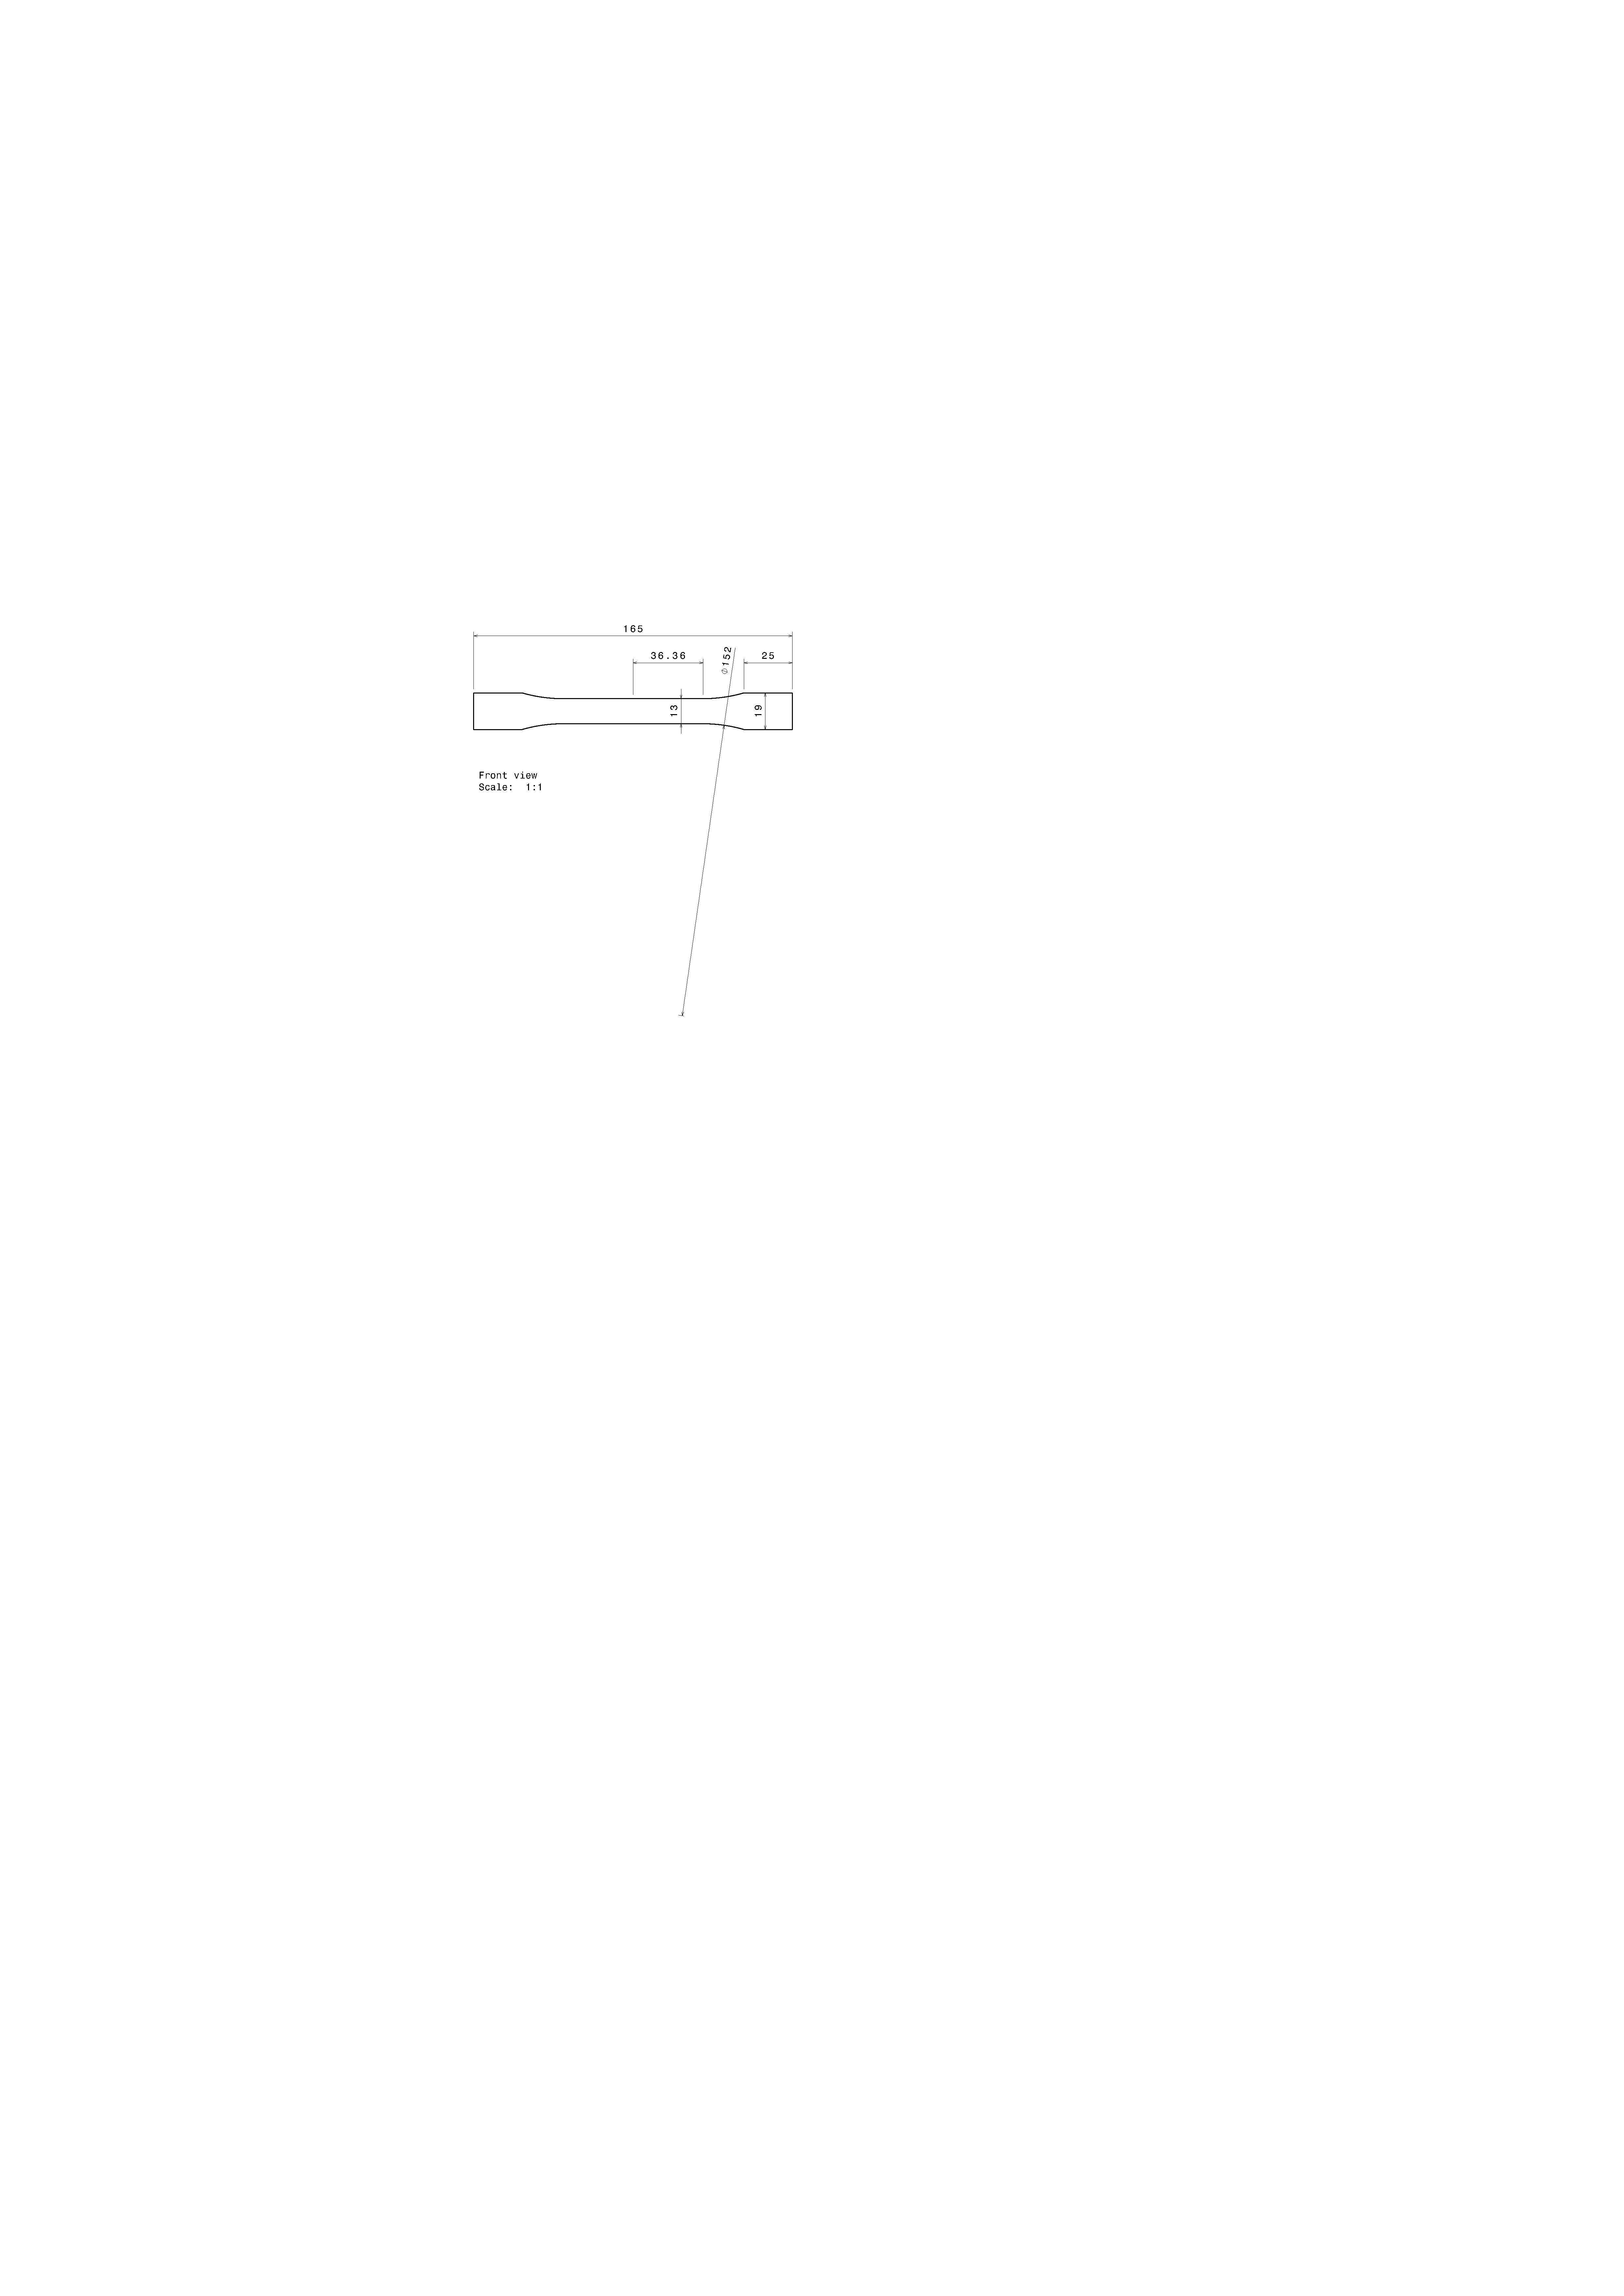
\includegraphics[ trim = {24cm 80cm 43cm 32cm}, clip , angle=0, scale=0.60 ]{imagens/Drawing1}
	\caption{Test parts CAD Draw.}
	\label{fig1}
\end{figure*}


From this scetch, a 3D model was created on a CAD software for printing (Figure \ref{fig2}). Such model was then exported as a STL file to the slicing software (Simplify3D), as seen on Fig.\ref{fig3}: 


\begin{figure*}[h!]
	\centering
	\begin{subfigure}[b]{0.5\textwidth}
		\centering
		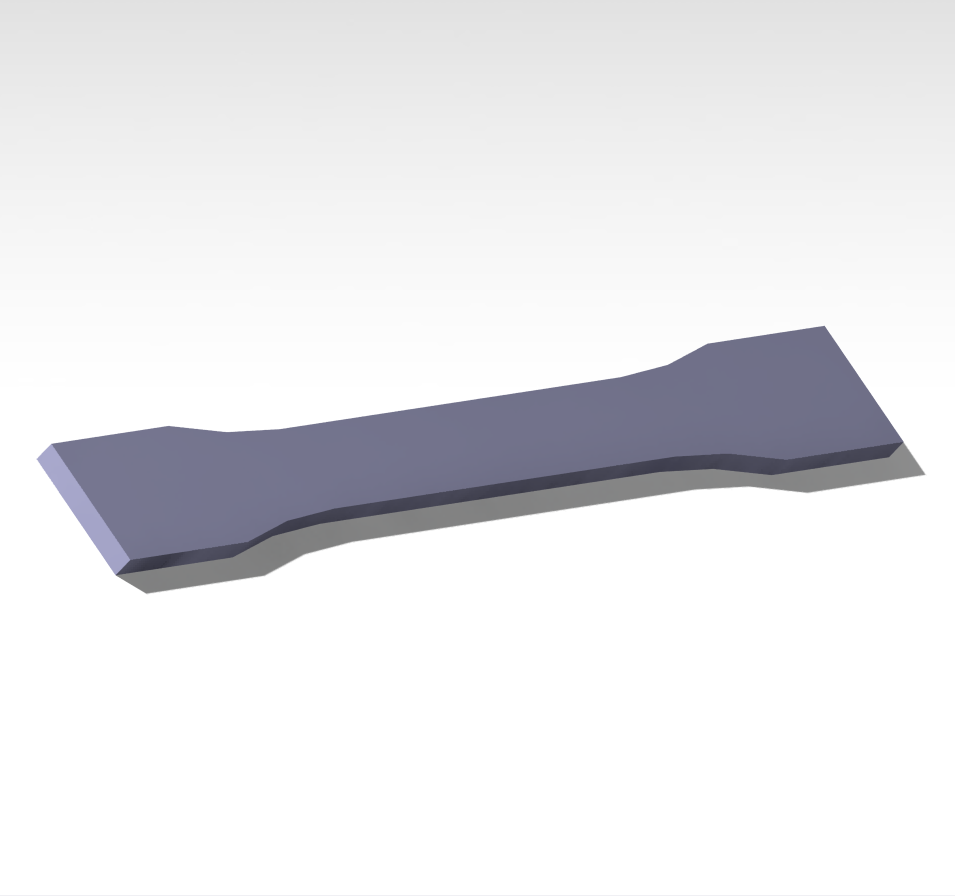
\includegraphics[ trim = {0 0 0 0}, clip , angle=0, scale=0.05 ]{imagens/renderizacao}
		\caption{CAD rendering.}
		\label{fig2}
	\end{subfigure}%
	~ 
	\begin{subfigure}[b]{0.5\textwidth}
		\centering
		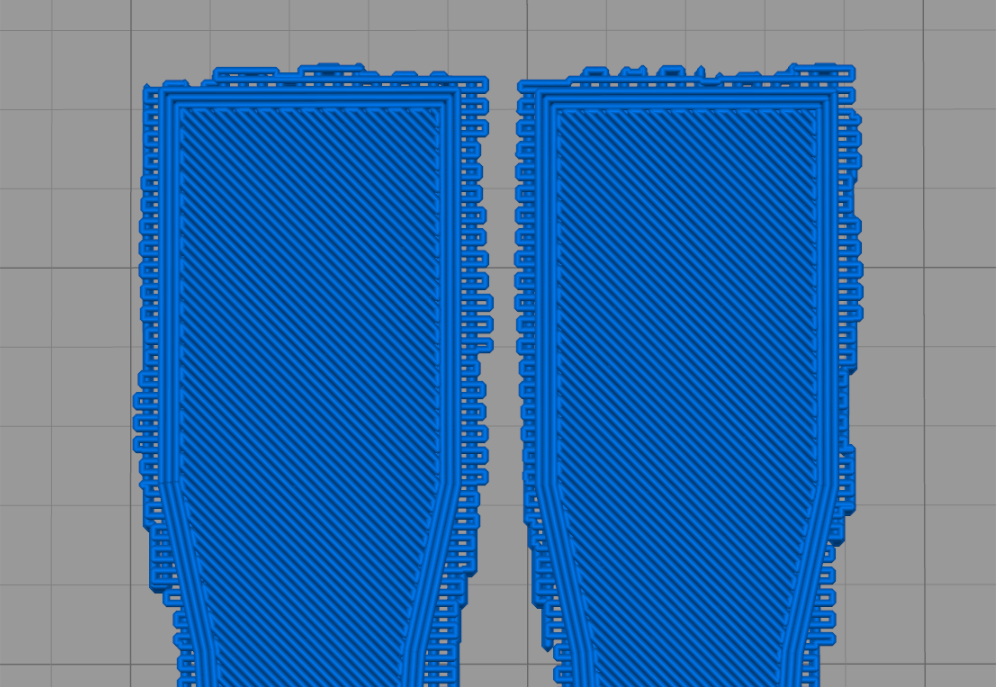
\includegraphics[ trim = {0cm 0cm 0 0cm}, clip , angle=0, scale=0.25 ]{imagens/simplify_zoom}
		\caption{Sliced part G code, read for printing.}
		\label{fig3}
	\end{subfigure}
	\caption{Modeling and slicing of the specimen for printing.}
\end{figure*}

In the image, is possible to see that the part was made on a support bed, in other words, not directly on the heated bed. Such method is to secure the z axis regularity on the printed part, as the fist layer printed directly over the heated plate has very different properties from the rest of the print, and due to these being very fin parts, such difference ends up not being 
negligible. 

Is important to point here the qualities that will be set to all the test specimens, parameters that will not be discussed on the present paper:

The infill of these parts were all set to $ 100 $ percent.


------> Oq por aqui?






%
%\begin{table}[!h]
%\centering
%\caption{Experimental results for flexural properties of CFRC-4HS and CFRC-TWILL composites. \protect\\Span/depth ratio = 35:1. Average results of 7 specimens.}
%\begin{tabular}{|c|c|c|}
%\hline
%Composite Properties & CFRC-TWILL & CFRC-4HS\\
%\hline
%Flexural Strength (MPa)$^{(1)}$ & 209$\pm$ 10 & 180 $\pm$  15\\
%\hline
%Flexural Modulus (GPa)$^{(1)}$ & 57.0 $\pm$ 2.8 & 18.0 $\pm$  1.3\\
%\hline
%Mid-span deflection at the failure stress (mm) & 2.15 $\pm$  1.90 & 6.40 $\pm$  0.25\\
%\hline
%\end{tabular}
%\\
%\begin{tabular}{p{11cm}ll}
%$^{(1)}$ measured at 25$^{o}$C & &
%\end{tabular}
%\label{tab1}
%\end{table}






\section{MATERIAL PROCEDURES}




----> Esperar experimento



\section{CONCLUSION}
The PETG (Polyethylene Terephthalate Glycol) is a good material for aerospace engineering, as its mechanical properties meet the project mechanical needs. 

As seen in the material experiments...








\section{ACKNOWLEDGEMENTS}
The authors would like to thank the following professors and institutions: Dr. Ruham Pablo Reis, Dr. Pedro Pio Rosa Nishida, Lmest (Structural Mechanics Laboratory), FEMEC (Mechanical engineering College), UFU (Federal University of Uberl\^andia) and, especially, EPTA(Propulsion and Aerospace Technology Team) for financial support.




\section{REFERENCES} 

\bibliographystyle{abcm}
\renewcommand{\refname}{}
\bibliography{bibfile}

\end{document}
